\section{The diagrammatic calculus of Demazure weaves}\label{sec:diagrammatic_weaves}

The diagrammatic calculus of weaves was initiated in \cite{CasalsZaslow}, and has subsequently been developed in a number of additional works, see e.g.~\cite{CGGJ24,CGGLSS25,CasalsWeng22,casals2023demazureweavesreducedplabic,casals2025comparingclusteralgebrasbraid,casals2025spectralnetworksbettilagrangians}. The goal of this first section is to introduce the diagrammatic calculus of Demazure weaves. For the sake of clarity, we focus on Demazure weaves on the 2-disk, and restrict to Type $A$, i.e.~to the special linear group. This particular case already illustrates many of the features and uses of weaves. There exists a more general theory of non-Demazure weaves, on an arbitrary surface, and for any simply-laced simple algebraic Lie group, cf.~\cite[Section 2]{CasalsZaslow} and \cite[Section 4]{CGGLSS25}. Two instances of Demazure weaves on the 2-disk in Type A are depicted in \Cref{fig:weave_intro_example}.\\

Let us thus fix $\mathsf{G}=\SL_n$, consider $\mbox{B}(\mathsf{G})$ the braid group associated to its $A_{n-1}$-Dynkin diagram and $\mbox{B}^+(\mathsf{G})$ the positive braid monoid. We denote by $\Br^+_n=\Br^+(\mathsf{G})$ the set of positive $n$-stranded braid words, i.e.~words on the positive Artin generators $\s_1,\ldots,\s_{n-1}$ of $\mbox{B}(\mathsf{G})$, which serve as representatives for elements in $\mbox{B}^+(\mathsf{G})$.

%%%%%%%%%%%%%%%%%%%%%%%%%%%%%%%%%%%%%%%%%%%%%%%%%%%%%%%%%%%%
%%%%%%%%%%%%%%%%%%%%%%%%%%%%%%%%%%%%%%%%%%%%%%%%%%%%%%%%%%%%
%%%%%%%%%%%%%%%%%%%%%%%%%%%%%%%%%%%%%%%%%%%%%%%%%%%%%%%%%%%%

\subsection{The definition of a Demazure weave}\label{ssec:primer_Demazure_weaves} Let us introduce Demazure weaves as follows:

\begin{definition}[Demazure weaves]\label{def:Demazure_weave}
Let $\beta,\beta'\in\Br^+_n$ be two positive braid words on $n$ strands. By definition, a Demazure weave $\w:\beta\lr\beta'$ is a sequence of positive braid words $\beta\to\beta_1\to\beta_2\to\cdots\to\beta'$, with $\beta_i\in\Br^+_n$, such that each move $\beta_j\to\beta_{j+1}$ is either a braid move in the positive braid monoid or the move $\s_i^2\to \s_i$.\sbs
\end{definition}

\noindent A Demazure weave $\w:\beta\lr\beta'$ where $\beta,\beta'\in\Br^+_n$ will be referred to as an $\SL_n$-weave if we need to emphasize the rank of $\mathsf{G}=\SL_n$. Note that both braid moves and $\s_i^2\to \s_i$ preserve the Demazure product $\delta(\beta)$ of $\beta$, as defined in \cite[Definition 3.1]{KnutsonMiller_04}, which partly justifies the choice of terminology.\\

\noindent A Demazure weave, as in \Cref{def:Demazure_weave}, can be depicted diagrammatically as follows. Let us draw a positive braid word $\s_{i_1}\cdots \s_{i_k}$ as a set of parallel vertical strands on the plane, with the $j$th strand from the left labeled by $\s_{i_j}$. Then the braid moves and the move $\s_i^2\to \s_i$ can be depicted as in \cref{fig:weaves_types_vertices}. More generally, \cref{fig:weave_intro_example} depicts an example of a Demazure weave $\w$ diagrammatically. In this diagrammatic presentation, each horizontal slice of a weave yields a braid word $\s_{i_1}\cdots \s_{i_k}$, cf.~\cref{fig:weave_intro_example}. %A core aspect of weave calculus are the Lusztig cycles of a Demazure weave, their intersection theory, and their behavior under weave equivalences and mutations, which we will momentarily summarize.

\begin{center}
	\begin{figure}[h!]
		\centering
		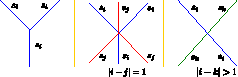
\includegraphics[scale=2.1]{figures/weaves_types_vertices.pdf}
		\caption{The three types of vertices allowed in the diagrammatic version of a weave $\w$. (Left) Trivalent vertex, where all edges are decorated with the same permutation $\s_i\in S_n$. It represents the move $\s_i^2\to \s_i$. (Center) Hexavalent vertex, with the edge decorations alternating between $\s_i,\s_j$ with $|i-j|=1$. It represents the braid move $\s_i\s_j\s_i\to \s_j\s_i\s_j$. (Right) Tetravalent vertex, with edge decorations as drawn with $|i-k|>1$. It represents the braid move $\s_i\s_k=\s_k\s_i$.}
		\label{fig:weaves_types_vertices}
	\end{figure}
\end{center}

\noindent When read from top to bottom, the diagram itself is often referred to as a Demazure weave. Considered as a planar graph, a Demazure weave admits the three types of vertices as in \cref{fig:weaves_types_vertices}, and the connected components of the complement of the vertices are said to be weave edges, cf.~\cite[Definition 2.1]{CasalsWeng22} or \cite[Section 2]{CasalsZaslow} for the general definition. The trivalent vertices of a weave $\w$ will be denoted $v_1,\dots,v_m$, ordered top-to-bottom, e.g.~with $v_i$ at height $i$. Each horizontal slice not intersecting a vertex determines a positive braid word by reading the weave edges left-to-right, as illustrated in \cref{fig:weave_intro_example}.\\

\begin{center}
	\begin{figure}[h!]
		\centering
		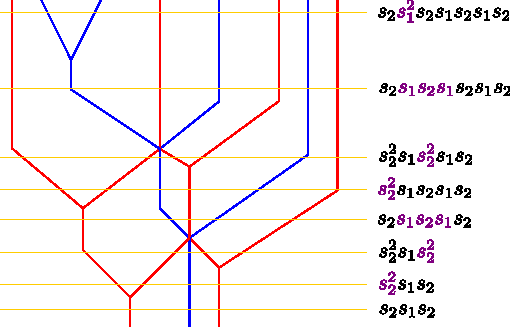
\includegraphics[scale=1]{figures/weave_intro_example.pdf}
		\caption{An instance of a Demazure weave $\w:\beta\lr\delta(\beta)$ from the 3-stranded braid word $\beta=\s_2\s_1(\s_1\s_2)^3$ to $\beta'=\s_2\s_1\s_2$, where blue weave edges are labeled by $s_1\in S_3$ and red weave edges by $s_2\in S_3$. Generic horizontal slices are depicted in yellow dashed lines, and the positive braid word associated to each such slice is written to its right. We have highlighted in purple the letters of each braid word to which the next move will be applied when scanning the Demazure weave downward.}
		\label{fig:weave_intro_example}
	\end{figure}
\end{center}

\begin{example}
For $\SL_2$, positive 2-stranded braid words are of the form $\beta=\sigma_1^n$ for some $n\in\N$. Thus Demazure weaves $\w:\sigma_1^n\lr\sigma_1$, up to equivalence, are in bijection with planar rooted binary trees, by reading the weave diagram bottom-to-top. For $\SL_n$ with $n\geq3$, the combinatorial study of weaves becomes significantly richer.\sbs
\end{example}


\begin{center}
	\begin{figure}[h!]
		\centering
		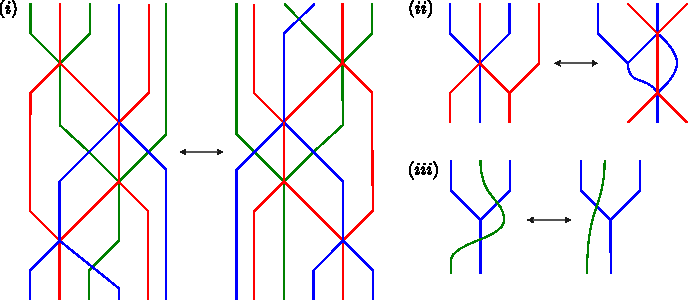
\includegraphics[scale=1.2]{figures/weave_equivalences2.pdf}
		\caption{A few weave equivalences, in all of them blue indicates $s_1\in S_4$, red $\s_2$, and green $\s_3$. $(i)$ This weave equivalence encodes a syzygy between braid moves, it is also known as the Zamolodchikov relation. $(ii)$ A weave equivalence known as the push-through move, as it allows for pushing trivalent vertices through hexavalent vertices. $(iii)$ A weave equivalence allowing for distant colors to pass through vertices of each other.}
		\label{fig:weave_equivalences}
	\end{figure}
\end{center}

%%%%%%%%%%%%%%%%%%%%%%%%%%%%%%%%%%%%%%%%%%%%%%%%%%%%%%%%%%%%
%%%%%%%%%%%%%%%%%%%%%%%%%%%%%%%%%%%%%%%%%%%%%%%%%%%%%%%%%%%%

\subsection{Weave equivalence and weave mutation}\label{sssec:weave_equivalences_mutations} There are two important diagrammatic operations on Demazure weaves: weave equivalences and weave mutations. Equivalences between weaves were first discussed in \cite[Theorem 1.1]{CasalsZaslow}, cf.~also \cite[Section 4]{CGGJ24}, and can be summarized as follows:

\begin{definition}[Weave equivalences]\label{def:weave_equivalences} By definition, a weave equivalence is either of the following four types of equivalences:
\begin{enumerate}[label=$(\roman*)$]
    \item Two weaves $\w,\w':\beta\to\beta'$ consisting only of braid moves are declared to be equivalent, see e.g.~\cref{fig:weave_equivalences}.(i).\\
    
    \item If $|i-j|=1$, the weaves $\w:\s_i\s_j\s_i\s_j\to \s_j\s_i\s_j\s_j\to \s_j\s_i\s_j$ and $\w':\s_i\s_j\s_i\s_j\to \s_i\s_i\s_j\s_i\to \s_i\s_j\s_i\to \s_j\s_i\s_j$  are declared to be equivalent, cf.~\cref{fig:weave_equivalences}.(ii).\\
    
    \item If $|i-j|\geq2$, the weaves $\w:\s_i\s_j\s_i\to \s_i\s_i\s_j\to \s_i\s_j\to \s_j\s_i$ and $\s_i\s_j\s_i\to \s_j\s_i\s_i\to \s_j\s_i$ are declared to be equivalent, cf.~\cref{fig:weave_equivalences}.(iii).\\

    \item Two weaves $\w,\w':\beta\to\beta'$ are declared to be equivalent if there exists a compactly supported isotopy of the plane, which is the identity at and above the north boundary of $\w$ and at and below the south boundary of $\w$, which brings $\w$ to $\w'$ through Demazure weaves.\\
\end{enumerate}
\noindent By definition, two weaves $\w,\w':\beta\to\beta'$ are said to be equivalent if there is a sequence of weave equivalences, as in $(i),(ii),(iii)$ and $(iv)$ above, starting at $\w$ and ending at $\w'$. $\sbs$
\end{definition}

\noindent Note that the equivalences in \Cref{def:weave_equivalences}.$(ii)$ and $(iii)$ are parameterized by rank $2$ subdiagrams of types $A_2$ and $A_1\times A_1$ respectively. A compactly supported isotopy as in \Cref{def:weave_equivalences}.$(iv)$ allows, for instance, to exchange the height of trivalent vertices that are far from each other, as depicted in \Cref{fig:Weave_HeightChangeEquivalence}.

\begin{center}
	\begin{figure}[ht]
		\centering
		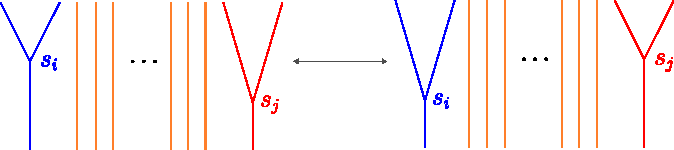
\includegraphics[scale=1.2]{figures/Weave_HeightChangeEquivalence.pdf}
		\caption{The local weave equivalence that exchanges the height of trivalent vertices, sometimes referred to as a pulley move. The weave lines in color orange indicate arbitrary and possibly different $\s_k$ labels, and the two labels $\s_i,\s_j$ are also arbitrary.\\}
        \label{fig:Weave_HeightChangeEquivalence}
	\end{figure}
\end{center}

\begin{comment}
\begin{example}
{\bf INSERT EXAMPLE OF TWO EQUIVALENT WEAVES HERE}
\end{example}
\end{comment}

There is a second important operation on weaves: weave mutation, which is not a weave equivalence. The notion of weave mutation was introduced in \cite[Section 4.8]{CasalsZaslow}.

\begin{center}
	\begin{figure}[h!]
		\centering
		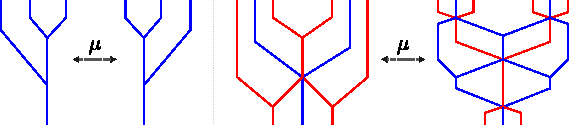
\includegraphics[scale=1.5]{figures/weave_mutation.pdf}
		\caption{(Left) An elementary weave mutation between the only two Demazure weaves $\w,\w':\s_1^3\to \s_1$. (Right) A more elaborate form of weave mutation, obtained by composing weave equivalences with an elementary weave mutation.}
		\label{fig:weave_mutation}
	\end{figure}
\end{center}

\begin{definition}[Weave mutation]\label{def:weave_mutation}
By definition, the two Demazure weaves $\w,\w':\s_i^3\to \s_i$ are said to be related by an elementary weave mutation, cf.~\cref{fig:weave_mutation} (left). In general, two weaves are said to be related by a weave mutation if they can be related by a sequence of weave equivalences, an elementary weave mutation, and another sequence of weave equivalences.    
\end{definition}

\noindent Two weaves that are mutation equivalent are not typically weave equivalent. For instance, the only two Demazure weaves from $\s_1^3\lr\s_1$, as drawn in \cref{fig:weave_mutation} (left), are not weave equivalent.

\begin{example}\label{ex:weave_mutation}
(1) \cref{fig:weave_mutation} (right) depicts two weaves $\w,\w':(\s_2\s_1\s_2)^2\to\s_2\s_1\s_2$ that are not equivalent to each other. Nevertheless, $\w,\w'$ are mutation equivalent to each other.\\

\noindent (2) \Cref{fig:weave_mutation_example} depicts two Demazure weaves $\w,\w':\s_2\s_1(\s_1\s_2)^3\lr \s_2\s_1\s_2$. These two weaves $\w,\w'$ are not weave equivalent. Instead they differ from each other by a sequence intertwining weave equivalences and two weave mutations.
\sbs
\end{example}

 \begin{center}
	\begin{figure}[ht!]
		\centering
		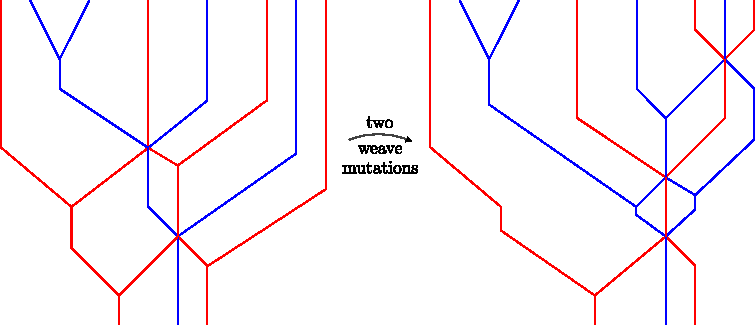
\includegraphics[scale=1]{figures/weave_mutation_example.pdf}
		\caption{Two instances of Demazure weaves $\w,\w':\beta\lr\beta'$ from $\beta=\s_2\s_1(\s_1\s_2)^3\in\Br^+_3$ to $\beta'=\s_2\s_1\s_2$, for \Cref{ex:weave_mutation}. Here the blue weave edges are labeled by $\s_1$ and red weave edges by $\s_2$.}
		\label{fig:weave_mutation_example}
	\end{figure}
\end{center}

\noindent The following result is \cite[Theorem 4.6]{CGGJ24}, which establishes the sufficiency of weave equivalences and weave mutation as a set of moves between Demazure weaves with fixed top and bottom boundaries:

\begin{theorem}
Let $\beta$ be a positive braid word. Then any two Demazure weaves $\w,\w':\beta\to\delta(\beta)$ are related by a sequence of equivalence moves and elementary mutations.\sbs
\end{theorem}

%%%%%%%%%%%%%%%%%%%%%%%%%%%%%%%%%%%%%
%%%%%%%%%%%%%%%%%%%%%%%%%%%%%%%%%%%%%
%%%%%%%%%%%%%%%%%%%%%%%%%%%%%%%%%%%%%

\subsection{Weave cycles and weighted braid words}\label{sssec:weave_cycles} Let $\w:\beta\to\beta'$ be a Demazure weave and $E(\w)$ its set of weave edges. The geometric notion of weave cycles was studied in \cite[Section 2]{CasalsZaslow} and \cite[Section 3.2]{CasalsWeng22}, see also \cite[Section 7.4]{CGGLSS25}. The following combinatorial notion of weave cycles was introduced in \cite[Section 4.4]{CGGLSS25}:

\begin{definition}[Weave cycles]\label{def:weave_cycles}
By definition, a weave cycle on $\w$ is a function $\g: E(\w) \to \Z_{\geq 0}$ that assigns a non-negative integer to each edge of the weave. The values of $\g$ are said to be the weights of the edges for the cycle $\g$.\sbs    
\end{definition}

In the same manner that each horizontal slice of a weave yields a braid word $\s_{i_1}\cdots \s_{i_k}$, cf.~\cref{fig:weave_intro_example}, given a weave cycle $\g$ and a horizontal slice we obtain a braid word $\s_{i_1}\cdots \s_{i_k}$ and a collection of non-negative integers ${\bf a}\coloneqq (a_1,\ldots,a_k)$, where $a_j\coloneqq \g(e_{i_j})$ is the weight of the $j$th weave edge $e_{i_j}\in E(\w)$ being intersected in that horizontal slice, corresponding to the letter $\s_{i_j}$ in the braid word $\s_{i_1}\cdots \s_{i_k}$. By definition, we refer to such a pair $(\s_{i_1}\cdots \s_{i_k},{\bf a})$ as a weighted braid word.

\begin{comment}
\begin{example}
{\bf INSERT EXAMPLE OF A WEAVE CYCLE.}
\end{example}
\end{comment}

%%%%%%%%%%%%%%%%%%%%%%%%%%%%%%%%%%%%%
%%%%%%%%%%%%%%%%%%%%%%%%%%%%%%%%%%%%%
%%%%%%%%%%%%%%%%%%%%%%%%%%%%%%%%%%%%%

\subsection{Lusztig cycles}\label{sssec:Lusztigcycles} Of particular importance are the following weave cycles associated to the trivalent vertices of the weave $\w$:

\begin{definition}[Lusztig cycles]\label{def:Lusztig_cycles}
Let $\w$ be a Demazure weave and $p\in\w$ a trivalent vertex. By definition, the Lusztig cycle $\g_p$ associated to $p$ is the unique weave cycle $\g_p: E(\mathfrak{W}) \to \Z_{\ge 0}$ such that:
\begin{itemize}
    \item[$(i)$] $\gamma_p(e_\mathsf{s})=1$ for the unique south edge $e_\mathsf{s}$ at the trivalent vertex $p$, and $\gamma_p(e)=0$ if $e$ is any weave edge that contains any points above $p$.\\
    
    \item[$(ii)$] At any other trivalent vertex with top edges $e_1,e_2$ and south edge $e$, $\g_p$ satisfies
    \begin{equation}\g_p(e)=\min(\gamma_p(e_1),\g_p(e_2))\,.\label{eq:3_move}\end{equation}
    
    \item[$(iii)$] For a 4-valent vertex  with top edges $e_1,e_2$ and  bottom edges $e_1',e_2'$, $\g_p$ satisfies
    \[(\g_p(e'_1),\g_p(e'_2))=(\g_p(e_2),\g_p(e_1))\,.\]
    
    \item[$(iv)$] For a 6-valent vertex  with top edges $e_1,e_2,e_3$ and bottom edges $e_1',e_2',e'_3$, $\g_p$ satisfies
    \begin{align*}
        \g_p(e'_1) & = \g_p(e_2)+\g_p(e_3)-\min(\gamma_p(e_1),\g_p(e_3))\,,\\
        \g_p(e'_2) & = \min(\gamma_p(e_1),\g_p(e_3))\,,\\
        \g_p(e'_3) & = \g_p(e_2)+\g_p(e_1)-\min(\gamma_p(e_1),\g_p(e_3))\,.
    \end{align*}
\end{itemize}
\sbs
%\noindent \qed
\end{definition}

\begin{center}
	\begin{figure}[h!]
		\centering
        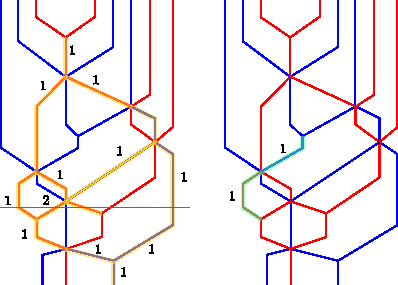
\includegraphics[scale=1.6]{figures/weave_Lusztigcycle_example.pdf}
		\caption{Two instances of Lusztig cycles on a Demazure weave $\w:(\s_1^2\s_2^2)^2\to \s_1\s_2\s_1$. (Left) The Lusztig cycle $\g_1$ associated to the first (top) trivalent vertex. The non-zero weave edges for $\g_1$ are highlighted in yellow, and the specific weight is written next to each weave edge. For instance, at the horizontal pink slice, the weighted braid word is $((\s_2^2\s_1)^2,(1,2,0,1,0,1))$. (Right) The Lusztig cycle $\g_2$ associated to the second trivalent vertex, with the non-zero weave edges for $\g_2$ highlighted in cyan.}\label{fig:weave_Lusztigcycle_example}
	\end{figure}
\end{center}

See \cref{fig:weave_Lusztigcycle_example} for two instances of Lusztig cycles; a non-highlighted edge (with no number) denotes weight 0. \cref{def:Lusztig_cycles} can also be described in terms of weighted braid words as follows. To construct $\g_p$, first consider a horizontal weave slice right below the height of $p$, which yields a certain braid word $\beta(p)\coloneqq \s_{i_1}\cdots \s_{i_{k(p)}}$ and assign the weights ${\bf a}(p)\coloneqq (0,0,\ldots,0,1,0,\ldots,0)$, where the only non-zero weight $1$ is assigned to the weave edge south of $p$. Then, propagate this weighted braid word $(\beta(p),{\bf a}(p))$ downwards by using the following rules for the weights:
\begin{multline}
\label{eq: lusztig trop}
\qquad \qquad \qquad \qquad \quad \Phi_1:(a_1,a_2)\mapsto \min(a_1,a_2), \quad \Phi_2:(a_1,a_2)\mapsto (a_2,a_1),\\ \qquad\qquad \Phi_3: (a_1,a_2,a_3)\mapsto  \left(a_2+a_3-\min(a_1,a_3),\min(a_1,a_3),a_1+a_2-\min(a_1,a_3)\right),
\end{multline}
where $\Phi_1$ is used at trivalent vertices, where the braid word changes according to $\s_i^2\lr \s_i$, $\Phi_2$ at tetravalent vertices, where the braid word changes as $\s_i\s_k=\s_k\s_i$ with $i,k$ non-adjacent, and $\Phi_3$ at hexavalent vertices, where the braid word changes via $\s_i\s_j\s_i=\s_j\s_i\s_j$ with $i,j$ adjacent.

\begin{remark} The downward propagation rules in \cref{eq: lusztig trop} above are referred to as tropical Lusztig rules, as they are obtained by tropicalizing the relations
\begin{multline*}
\label{eq: lusztig trop2}
\qquad \qquad \qquad \qquad \quad x_i(t_1)x_i(t_2)=x_i(t_1+t_2), \quad x_i(t_1)x_k(t_2)=x_k(t_2)x_i(t_1),\\ x_i(t_1)x_j(t_2)x_i(t_3)=
x_j\left(\frac{t_2t_3}{t_1+t_3}\right)x_i(t_1+t_3)x_j\left(\frac{t_1t_2}{t_1+t_3}\right), \hskip 2.8cm
\end{multline*}
\noindent where $x_i(t)\coloneqq \exp(E_{i,i+1}t)$ is the 1-parameter subgroup in $\on{SL}_n$ corresponding to the positive simple root $\alpha_i$, cf.~\cite[Proposition 2.5]{Lusztig}. Here the indices $i,j$ are adjacent, and $i,k$ non-adjacent, in the Dynkin diagram.\sbs
\end{remark}

\noindent For reasons related to cluster algebras, to become clearer later, we introduce the following notation:

\begin{definition}[Mutable and frozen Lusztig cycles]\label{def:mutable_frozen}
A Lusztig cycle $\g$ in a Demazure weave $\w$ is said to be mutable if its weights vanish, i.e.~$\g(e)=0$, on all edges $e\in\w$ of the south boundary of $\w$; it is otherwise said to be frozen.\sbs
\end{definition}
It is important to emphasize that the adjective {\it mutable} in \Cref{def:mutable_frozen} does not refer to the Lusztig cycle itself being able to undergo a weave mutation, as this might not be the case. The adjective refers to the notion of {\it mutable} vertex of a quiver and its corresponding cluster variable.

%%%%%%%%%%%%%%%%%%%%%%%%%%%%%%%%%%%%%
%%%%%%%%%%%%%%%%%%%%%%%%%%%%%%%%%%%%%
%%%%%%%%%%%%%%%%%%%%%%%%%%%%%%%%%%%%%

\subsection{Intersection form on weave cycles}\label{ssec:intersection_cycles} Let us now introduce a skew-symmetric bilinear form on the set of weave cycles. Given two weave cycles $\g,\g': E(\w)\to\Z_{\geq0}$ on a weave $\w$, not necessarily Lusztig cycles, we now define their intersection number $\sharp_{\w}(\g \cdot \g')$ as a sum of local contributions from intersections at the 3-valent vertices, at the 6-valent vertices, and an additional boundary intersection term.

\begin{center}
	\begin{figure}[h!]
		\centering
        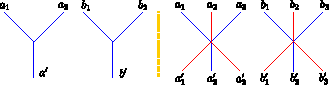
\includegraphics[scale=2]{figures/weaves_types_vertices_trivalent_intersection.pdf}
		\caption{(Left) Two weave cycles near a trivalent vertex, with their weights indicated on each edge. Their local intersection at the trivalent vertex is computed via the determinant in \Cref{def:locint_3valent}. (Right) Two weave cycles near a hexavalent vertex, with their weights indicated on each edge. Their local intersection at this hexavalent vertex is computed via \Cref{def:locint_6valent}.}\label{fig:weaves_types_vertices_trivalent_intersection}
	\end{figure}
\end{center}

\begin{definition}[Local intersection at 3-valent vertex]\label{def:locint_3valent} Let $\w$ be a Demazure weave, $v\in\w$ a trivalent vertex, and $\g,\g': E(\w)\to\Z_{\geq0}$ two weave cycles as in \Cref{fig:weaves_types_vertices_trivalent_intersection} (left). That is, $\g$ $($resp.~$\g')$ has weights $a_1,a_2$ $($resp.~$b_1,b_2)$ on the northwest and northeast edges of the trivalent vertex $v$, respectively, and weight $a'$ $($resp.~$b')$ on the south edge. By definition, the local intersection number of $\g,\g'$ at $v$ is
$$
\sharp_{v}(\g\cdot \g'):=\left|
\begin{matrix}
1 & 1 & 1\\
a_1 & a' & a_2\\
b_1 & b' & b_2\\
\end{matrix}
\right|.
$$
\sbs
\end{definition}

%CHECK SIGNS {Jos\'e: Signs seem correct.}
%\begin{example}
%Suppose that $(a_1,a',a_2)=(0,1,0)$. Then 
%$\sharp(C\cdot \g')=b_2-b_1$.
%\end{example}

\begin{definition}[Local intersection at 6-valent vertex]\label{def:locint_6valent} Let $\w$ be a Demazure weave, $v\in\w$ a hexavalent vertex, and $\g,\g': E(\w)\to\Z_{\geq0}$ two weave cycles as in \Cref{fig:weaves_types_vertices_trivalent_intersection} (right).
That is, $\g$ $($resp.~$\g')$ has weights $a_1,a_2,a_3$ $($resp.~$b_1,b_2,b_3)$ on the northwest, north and northeast edges of the 6-valent vertex $v$, and weights $a'_1,a'_2,a'_3$ $($resp.~$b'_1,b'_2,b'_3)$ on the southwest, south and southeast edges of $v$. By definition, the local intersection number of $\g,\g'$ at $v$ is
$$
\sharp_{v}(\g\cdot \g'):=\frac{1}{2}\left(
\left|
\begin{matrix}
1 & 1 & 1\\
a_1 & a_2 & a_3\\
b_1 & b_2 & b_3\\
\end{matrix}
\right|-
\left|
\begin{matrix}
1 & 1 & 1\\
a'_1 & a'_2 & a'_3\\
b'_1 & b'_2 & b'_3\\
\end{matrix}
\right|
\right).
$$
\sbs
\end{definition}

\begin{center}
	\begin{figure}[h!]
		\centering
        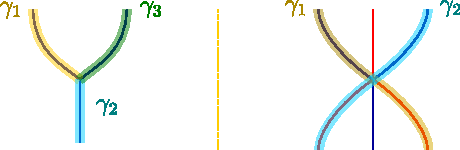
\includegraphics[scale=1]{figures/example_local_intersection.pdf}
		\caption{(Left) Three weave cycles $\g_1,\g_2,\g_3$ near a trivalent vertex: they are each declared to have weight 0 on every edge except for the edge highlighted in their corresponding color, where they have weight 1. (Right) Two weave cycles $\g_1,\g_2$ near a hexavalent vertex: each is declared to have weight 0 on every edge except for the edges highlighted in their corresponding color, where they have weight 1. Their intersections are computed in \Cref{ex:local_intersection}.}\label{fig:example_local_intersection}
	\end{figure}
\end{center}

\begin{example}\label{ex:local_intersection} (1) Consider the cycles $\g_1,\g_2,\g_3$ depicted in \Cref{fig:example_local_intersection} (left) near a trivalent vertex $v$. Specifically, $\g_1$ has weight 1 on the northwest edge of the trivalent vertex, and weight 0 elsewhere. Similarly, $\g_2$ has weight 1 on the south edge of the trivalent vertex, and weight 0 elsewhere, and $\g_3$ has weight 1 on the northeast edge of the trivalent vertex, and weight 0 elsewhere. By \cref{def:locint_3valent}, their local intersections are
$$\sharp_{v}(\g_1\cdot \g_2)=1,\quad \sharp_{v}(\g_2\cdot \g_3)=1,\quad\sharp_{v}(\g_3\cdot \g_1)=1.$$

\noindent Note that their local self-intersections $\sharp_{v}(\g_i\cdot \g_i)=0$ at $v$ all vanish, $i\in[1,3]$, as the matrix in \cref{def:locint_3valent} has two identical rows and thus the determinant vanishes.\\

\noindent (2) Consider the cycles $\g_1,\g_2$ depicted in \Cref{fig:example_local_intersection} (right) near a hexavalent vertex $v$. Specifically, $\g_1$ has weight 1 on the northwest and southeast edges of $v$, and weight 0 otherwise, and $\g_2$ has weight 1 on the northeast and southwest edges of  $v$, and weight 0 otherwise. By \Cref{def:locint_6valent}, their local intersection at $v$ is
$$\sharp_{v}(\g_1\cdot \g_2)=-1.$$
\sbs
\end{example}

\begin{definition}[Intersection form on weave cycles]\label{def:intersection_number}
Let $\w$ be a Demazure weave and $\g,\g':E(\w)\to\Z_{\geq0}$ two weave cycles whose weights at the top and bottom edges of $\w$ vanish. By definition, the intersection number $\langle\g, \g'\rangle\in\mathbb{Q}$ of $\g$ and $\g'$ is
\begin{equation}\label{eq:intersection_form}
\langle\g, \g'\rangle := \sum_{\mbox{\tiny $v$ 3-valent}}\sharp_{v}(\g \cdot \g') + \sum_{\mbox{\tiny $v$ 6-valent}}\sharp_{v}(\g\cdot \g').
\end{equation}
\sbs
\end{definition}

\noindent It follows from \Cref{def:locint_3valent} and \Cref{def:locint_6valent} that the intersection number is skew-symmetric:
$$\langle\g, \g'\rangle = -\langle\g', \g\rangle.$$
Also, the intersection number $\langle\g, \g'\rangle$ is an integer when $\g, \g'$ are both mutable Lusztig cycles, as in \Cref{def:Lusztig_cycles}. In particular, the collection of mutable Lusztig cycles endowed with this skew-symmetric intersection form determines an intersection quiver (with no frozen vertices). The intersection numbers from \Cref{def:intersection_number} define a skew-symmetric intersection form, by extending bilinearly, on the lattice of $\Z$-valued weave cycles.

\begin{example}\label{ex:Lusztig_cycles}
Consider the two weaves in \cref{fig:weave_intro_example2}, as in \Cref{ex:weave_mutation}.(2) above. For each of the weaves, \Cref{fig:weave_intro_example2} depicts the three Lusztig cycles associated to the top vertices and their corresponding intersection quivers, computed via \Cref{def:intersection_number}. Specifically, their intersection matrices are
$$(\langle\g_i, \g_j\rangle)=\begin{pmatrix}
0 & 1 & 0\\
-1 & 0 & 1\\
0 & -1 & 0
\end{pmatrix},\qquad (\langle\g'_i, \g'_j\rangle)=\begin{pmatrix}
0 & -1 & 0\\
1 & 0 & 1\\
0 & -1 & 0
\end{pmatrix},\quad \mbox{for }i,j\in[1,3].$$
respectively for the Lusztig cycles $\gamma_1,\gamma_2,\gamma_3$ on the left weave $\w$, and the Lusztig cycles $\gamma'_1,\gamma'_2,\gamma'_3$ on the right weave $\w'$.\sbs
\end{example}
 
 \begin{center}
	\begin{figure}[ht!]
		\centering
		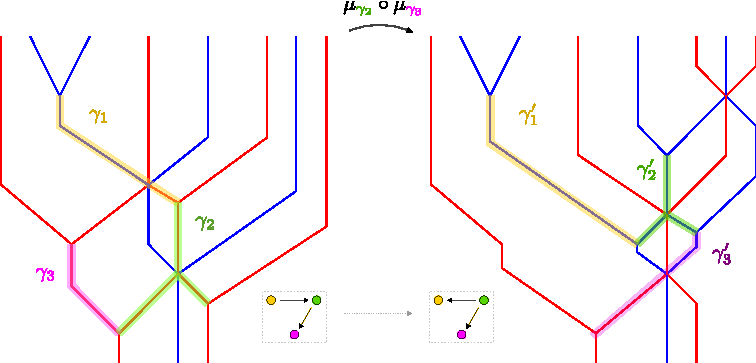
\includegraphics[scale=1]{figures/weave_intro_example2}
		\caption{Two instances of Demazure weaves. (Left) The mutable Lusztig cycles $\gamma_1,\gamma_2,\gamma_3$ for $\w$ are highlighted in yellow, green and pink respectively, and their intersection quiver is displayed in the square box at the lower right of $\w$.  (Right) The weave $\w'$ obtained from $\w$ by performing weave mutations along the Lusztig cycles $\gamma_3$ and $\gamma_2$, in this order. Its corresponding Lusztig cycles $\gamma'_1,\gamma'_2,\gamma'_3$ are also highlighted and their intersection quiver is displayed to the lower left of $\w'$.}
		\label{fig:weave_intro_example2}
	\end{figure}
\end{center}

\begin{remark}[Boundary intersections]\label{rmk:boundary_intersections}
\Cref{def:locint_3valent} and \Cref{def:locint_6valent} suffice for computing intersections between weave cycles whose weights at the top and bottom edges of the weave are zero, as in \Cref{def:intersection_number}. This suffices for most applications, as it concerns the mutable part of the intersection quiver, cf.~\Cref{def:mutable_frozen}. Nevertheless, there is in general an intersection contribution $\sharp_{\partial}(\g\cdot \g')$ from the top and bottom boundary edges of $\w$ as well, see e.g.~\cite[Section 4.6]{CGGLSS25}. For any two weave cycles $\g,\g'$, possibly not vanishing at the boundary edges of $\w$, we can take into account this boundary intersection contribution for $\g,\g'$ and define their intersection as
\[
\langle\g, \g'\rangle := \sharp_{\partial}(\g\cdot \g')+\sum_{\mbox{\tiny $v$ 3-valent}}\sharp_{v}(\g \cdot \g') + \sum_{\mbox{\tiny $v$ 6-valent}}\sharp_{v}(\g\cdot \g').
\]
\sbs
\end{remark} 

\begin{comment}
\color{orange}
Recall that we denote the Cartan subgroup of $\G$ by $T$. Denote by $X$ and $X^\vee$ the lattices of characters and cocharacters of $T$. Consider the perfect pairing  
\begin{equation}
\label{22.7.20.1}
(\cdot, \cdot): ~ X \times X^\vee \longrightarrow \mathbb{Z}.
\end{equation}
Let $\{\alpha_i\}$ and $\{\alpha_i^\vee\}$ be the set of simple roots and simple coroots, indexed by the vertices in $\dynkin$.
Now given a braid word $\beta=\sigma_{i_1}\cdots\sigma_{i_k}$, we consider the following sequences  of roots and coroots (cf. \cite{CLS}):
\begin{equation}
\label{eq: def gamma}
\rho_j:= s_{i_1}\cdots s_{i_{j-1}}(\alpha_{i_j}), \qquad \rho_j^\vee:=s_{i_1}\cdots s_{i_{j-1}}(\alpha_{i_j}^\vee),\qquad \forall 1\leq j \leq k.
%\rho_1 := \alpha_{i_1},~~ \rho_2 := s_{i_{1}}(\alpha_{i_2}),~~ \ldots,~~ \rho_{k} := s_{i_{1}}\cdots s_{i_{k-1}}(\alpha_{i_k}).
%\gamma_k=\alpha_{i_k},\ \gamma_{k-1}=s_{i_{k-1}}(\alpha_{i_k}),\ldots, \gamma_1=s_{i_1}s_{i_{2}}\cdots s_{i_{k-1}}(\alpha_{i_k}).
\end{equation}
Note that $\rho_{j} = s_{i_{1}}\cdots s_{i_{j}}(-\alpha_{i_j})$.  For a weave $\fW$ and a cycle $C$, such that $\beta$ appears as a horizontal section of $\fW$, we denote by $c_j$ the weight of $C$ on the $j$-th letter of $\beta$.

%{\color{red} Linhui: Definition 4.21 and the definition of p-matrices should also be modified}
\begin{definition}
\label{def: boundary intersection}
Let $\fW$ be a weave and $C, C':E(\fW)\to\Z_{\geq0}$ cycles and $\beta = \sigma_{i_{1}}\cdots \sigma_{i_{r}}$  a braid word which is a horizontal section of $\fW$. By definition, the boundary intersection $\sharp_{\beta}(C\cdot C')$ of $C,C'$ at $\beta$ is 
\[
\sharp_{\beta}(C\cdot C'):=\frac{1}{2}\sum_{i,j = 1}^{r}\sign(j-i)c_{i}c'_{j}\cdot(\rho_{i}, \rho_{j}^\vee)
\]%\langle \gamma_C,\gamma_{C'}\rangle
where $(\cdot, \cdot)$ is the pairing defined via \eqref{22.7.20.1}, and
\[
\sign(k) = \begin{cases} 1 & \mbox{if }k >0, \\ 0 & \mbox{if }k = 0, \\ -1 & \mbox{if }k < 0. \end{cases}
\]
\end{definition}

\begin{remark}
In Definition \ref{def: boundary intersection} and throughout this section we are assuming that the group $\G$ is of simply laced type. For non-simply laced type Definition \ref{def: boundary intersection} has to be modified to take into account cycles for the Langlands dual group $\G^{\vee}$ of $\G$, see Section \ref{sec: non simply laced defs} and in particular \eqref{eq: boundary intersection non simply laced} below.
\end{remark}

\begin{definition}\label{def:quiver}
Let $\fW$ be a Demazure weave. By definition, the quiver $Q_{\fW}$ is the quiver whose vertices are (in bijective correspondence with) the trivalent vertices of $\fW$, and whose adjacency matrix is given by%
\[
\varepsilon_{v,v'} := \sharp_{\fW}(\g_{v}\cdot \g_{v'}) + \sharp_{\delta(\beta)}(\g_{v} \cdot \g_{v'}).
\]
where $\delta(\beta)$ is the bottom slice of the weave $\fW$.%the intersection number $\sharp_{\fW}(\g_{v}\cdot \g_{v'})$ at the entry associated to two vertices $v,v'\in\fW$.
\end{definition}

\begin{remark}
The entries  $\varepsilon_{v,v'}$ in Definition \ref{def:quiver} are always half-integers but not necessarily integers. Note also that the boundary intersection terms for $\varepsilon_{v,v'}$ vanish for cycles $\gamma_v,\gamma_{v'}$ (either of) which do not reach the bottom part of the weave: in the language of Subsection \ref{ssec:frozen}, the boundary intersection terms only appear between frozen vertices, and the weights of arrows involving a mutable vertex are always integers. 
\end{remark}
\color{black}
\end{comment}
%%%%%%%%%%%%%%%%%%%%%%%%%%%%%%%%%%%%%
%%%%%%%%%%%%%%%%%%%%%%%%%%%%%%%%%%%%%
%%%%%%%%%%%%%%%%%%%%%%%%%%%%%%%%%%%%%

\subsection{Dual Lusztig cycles}\label{sssec:dual_Lusztigcycles} Let $\w:\beta\lr\delta(\beta)$ be a Demazure weave. The Lusztig cycles $\{\g_v\}$ of $\w$, indexed by the trivalent vertices of $\w$ as in \Cref{def:Lusztig_cycles}, are an important set of weave cycles of $\w$. Equally relevant is the dual collection $\{\rho_v\}$ of dual Lusztig cycles, dual with respect to the intersection product introduced in \Cref{ssec:intersection_cycles}. In fact, given $\{\g_v\}$ and the skew-symmetric product, it follows from induction and the normalized propagation rules that there exists a distinguished family of weave cycles $\{\rho_v\}$ that vanish at the bottom boundary of $\w$ such that
\begin{equation}\label{eq:duality}
\langle \g_v,\rho_{v'}\rangle =\delta_{v,v'}\,.
\end{equation}

\noindent Specifically, such dual Lusztig cycles $\{\rho_v\}$ for a Demazure weave, which are also indexed by the trivalent vertices of $\w$, can be constructed as follows:


\begin{definition}[Dual Lusztig cycles]\label{def:dual_Lusztig_cycles}
Let $\w$ be a Demazure weave, $\{\g_v\}$ its collection of Lusztig cycles, and $v\in\w$ a trivalent vertex. By definition, the dual Lusztig cycle $\r_v$ associated to $v$ is the unique weave cycle $\r_v: E(\w) \to \Z_{\ge 0}$ such that:\\
\begin{itemize}
    \item[$(i)$] The weights of $\r_v$ at the edges of $v$ are:
    $$\r_v(e_\mathsf{ne})=1,\quad \r_v(e_\mathsf{nw})=0,\quad \r_v(e_\mathsf{s})=0,$$
    where $e_\mathsf{ne}$ denotes the unique northeast edge at the trivalent vertex $v$, and $e_\mathsf{nw}$ and $e_\mathsf{s}$ the unique northwest and south edges at $v$. In addition,
    $$\r_v(e)=0$$
    for any weave edge $e$ that contains any points below $v$.\\
    
    \item[$(ii)$] At a trivalent vertex $p$ different from $v$, where $e_\mathsf{nw}$, $e_\mathsf{ne}$ and $e_\mathsf{s}$ are respectively the northwest, northeast and south edges of $p$, the weights of the weave cycle $
    \rho_v$ are
    \begin{equation}\label{eq:dualLusztigcycle_trivalentrule_left}
    \rho_v(e_\mathsf{nw})=\rho_v(e_\mathsf{s})+\textcolor{green}{\max(-\langle (\rho_v)_{<p},\g_p\rangle,0)},\quad \rho_v(e_\mathsf{ne})=\rho_v(e_\mathsf{s})+\textcolor{blue}{\max(\langle (\rho_v)_{<p},\g_p\rangle,0)},
    \end{equation}
    where $(\rho_v)_{<p}$ denotes the weave cycle obtained by restricting $\rho_v$ to the entire weave below the trivalent vertex $p$.\\
    
    \item[$(iii)$] For a 4-valent vertex  with top edges $e_1,e_2$ and  bottom edges $e_1',e_2'$, $\r_v$ satisfies
    \[(\r_v(e'_1),\r_v(e'_2))=(\r_v(e_2),\r_v(e_1))\,.\]
    
    \item[$(iv)$] For a 6-valent vertex  with top edges $e_1,e_2,e_3$ and bottom edges $e_1',e_2',e'_3$, $\r_v$ satisfies
    \begin{align*}
        \r_v(e'_1) & = \r_v(e_2)+\r_v(e_3)-\min(\r_v(e_1),\r_v(e_3))\,,\\
        \r_v(e'_2) & = \min(\r_v(e_1),\r_v(e_3))\,,\\
        \r_v(e'_3) & = \r_v(e_2)+\r_v(e_1)-\min(\r_v(e_1),\r_v(e_3))\,.
    \end{align*}
\end{itemize}
\sbs
%\noindent \qed
\end{definition}

\noindent The genuine difference between dual Lusztig cycles and Lusztig cycles is in \Cref{def:dual_Lusztig_cycles}.(i) and (ii). We often refer to the terms highlighted in green and blue in \eqref{eq:dualLusztigcycle_trivalentrule_left} as correction terms. Indeed, \Cref{def:dual_Lusztig_cycles}.(iii) and (iv) are identical to the rules of \Cref{def:Lusztig_cycles} at 4-valent and 6-valent vertices. A few comments on \Cref{def:dual_Lusztig_cycles}:

\begin{enumerate}
    \item For each trivalent vertex $v\in\w$, the non-zero weights of the Lusztig cycle $\g_v$ all lie below $v$. In a sense, $\g_v$ propagates downwards: it can be constructed by starting at $v$ and assigning non-zero weights to certain weave edges below $v$ according to \Cref{def:Lusztig_cycles}. In contrast, the non-zero weights of the dual Lusztig cycle $\r_v$ all lie above $v$. Similarly, $\r_v$ can be considered to propagate upwards: it can be constructed by starting at $v$ and assigning non-zero weights to certain weave edges above $v$ according to \Cref{def:dual_Lusztig_cycles}.\\

    \item By construction, specifically \eqref{eq:dualLusztigcycle_trivalentrule_left}, the Lusztig cycles $\{\g_v\}$ and the dual Lusztig cycles $\{\rho_v\}$ satisfy the duality in \eqref{eq:duality},  where we have used the intersection product from \Cref{ssec:intersection_cycles}. Indeed, suppose $v'$ is a trivalent vertex below $v$ and $e_\mathsf{s}$ is the south edge of $v$. Then
    \begin{equation*}
\begin{split}
\langle \g_v,\rho_{v'}\rangle & = \langle \g_v,(\rho_{v'})_{<v}\rangle+\sharp_{v}(\g_v \cdot \r_{v'}) \\
  & \stackrel{\eqref{eq:dualLusztigcycle_trivalentrule_left}}{=} \langle \g_v,(\rho_{v'})_{<v}\rangle+\left|
\tiny\begin{matrix}
1 & 1 & 1\\
0 & 1 & 0\\
\r(e_\mathsf{s})+\textcolor{green}{\max(\langle \g_v,(\rho_{v'})_{<v}\rangle,0)} & \r(e_\mathsf{s}) & \r(e_\mathsf{s})+\textcolor{blue}{\max(-\langle \g_v,(\rho_{v'})_{<v}\rangle,0)}\\
\end{matrix}
\right|\\
\normalsize
 & = \langle \g_v,(\rho_{v'})_{<v}\rangle+\r_{v'}(e_\mathsf{s})+\max(-\langle \g_v,(\rho_{v'})_{<v}\rangle,0) - \r_{v'}(e_\mathsf{s})-\max(\langle \g_v,(\rho_{v'})_{<v}\rangle,0)\\
 & = 0.
\end{split}
\end{equation*}
    
\noindent In the last equality we used that $a=[a]_+-[-a]_+$, where we denote $[a]_+:=\max(a,0)$. The identity \eqref{eq:duality} partially justifies the adjective {\it dual} for dual Lusztig cycles.\\

    \item Note also that \eqref{eq:dualLusztigcycle_trivalentrule_left} implies that $\rho_v$ behaves like a Lusztig cycle near any trivalent vertex $p$ above $v$. Indeed, near such $p$, with edges $e_\mathsf{nw},e_\mathsf{ne}$ and $e_\mathsf{s}$, the dual Lusztig cycle $\rho_v$ satisfies
     $$\rho_v(e_\mathsf{s})=\min(\rho_v(e_\mathsf{nw}), \rho_v(e_\mathsf{ne}))$$
     as at least one of the correction terms in \eqref{eq:dualLusztigcycle_trivalentrule_left} is zero.
\end{enumerate}

\begin{remark}
The notion of ``propagation'' of a weave cycle, either downwards or upwards, as emphasized in $(1)$ above, can be conceptualized in categorical terms by using certain left adjoint induction functors and semitwists, cf.~\cite[Sections 7.3 \& 9.4]{CasalsChrist}. In addition, there is a categorical explanation for the intersection term $\langle (\rho_v)_{<p},\g_p\rangle$ in $\eqref{eq:dualLusztigcycle_trivalentrule_left}$, in terms of Ext groups, cf.~\cite[Section 9.3]{CasalsChrist} and \eqref{eq:y} below.\sbs
\end{remark}

\noindent An interesting combinatorial fact about dual Lusztig cycles is that the northwest correction term in \eqref{eq:dualLusztigcycle_trivalentrule_left} always vanishes:

\begin{proposition}[Right-veering property of dual Lusztig cycles]\label{prop:rightveering} Let $\w:\beta\lr\delta(\beta)$ be a Demazure weave, $v\in\w_3$ a trivalent vertex and $\rho_v$ its dual Lusztig cycle. Then, for any other trivalent vertex $p\in\w_3$, 
$$\rho_v(e_{\mathsf{nw}})=\rho_v(e_{\mathsf{s}})$$
where $e_{\mathsf{nw}},e_{\mathsf{s}}$ denote the northwest and south edges of $p$.\sbs
\end{proposition}

\noindent That is, \Cref{prop:rightveering} is equivalent to the fact that the green correction term in \eqref{eq:dualLusztigcycle_trivalentrule_left} in \Cref{def:dual_Lusztig_cycles}.(ii) always vanishes. In view of \Cref{prop:rightveering}, one can in practice directly substitute \eqref{eq:dualLusztigcycle_trivalentrule_left} by
  \begin{equation}\label{eq:dualLusztigcycle_trivalentrule_left2}
    \rho_v(e_\mathsf{nw})=\rho_v(e_\mathsf{s}),\quad \rho_v(e_\mathsf{ne})=\rho_v(e_\mathsf{s})+\textcolor{blue}{\langle (\rho_v)_{<p},\g_p\rangle}
    \end{equation}
in \Cref{def:dual_Lusztig_cycles}, implicitly understanding that it is a non-trivial fact that $\langle (\rho_q)_{<v},\g_v\rangle$ is always non-negative. A proof of such non-negativity, and thus of \Cref{prop:rightveering}, follows from the equality
\begin{equation}\label{eq:y}
\langle (\rho_q)_{<v},\g_v\rangle = \on{dim}\on{Ext}^1(S_{p},\on{tot}(\mathcal{C}_{\ast\geq b})),
\end{equation}
where the terms on the right hand side of \eqref{eq:y} are explained in \cite[Section 9]{CasalsChrist}. In a nutshell, the right hand side of \eqref{eq:y} is the dimension of an $\on{Ext}^1$ group between certain dg-modules over the derived preprojective algebra, which are used in the additive categorifications introduced in \cite[Theorems A\&B]{CasalsChrist}. In particular, since dimensions are non-negative, it follows that $\langle (\rho_q)_{<v},\g_v\rangle$ is non-negative. In view of \Cref{prop:rightveering}, from now on we adopt \Cref{def:dual_Lusztig_cycles} always using \eqref{eq:dualLusztigcycle_trivalentrule_left2} instead of \eqref{eq:dualLusztigcycle_trivalentrule_left}.

\begin{remark}\label{rmk:rightveering_combinatorial} It would be wonderful to have a combinatorial proof of \Cref{prop:rightveering}. The challenge is that $\langle (\rho_q)_{<v},\g_v\rangle$ is a sum of local contributions and, typically, these contributions are both positive and negative. Thus, the difficulty lies in finding a combinatorial argument for a global cancellation, whereby all the negative terms, which come from some of the hexavalent vertices, actually must be cancelled by the positive terms coming from the trivalent and some of the other hexavalent vertices.\sbs
\end{remark}



\begin{center}
	\begin{figure}[h!]
		\centering
        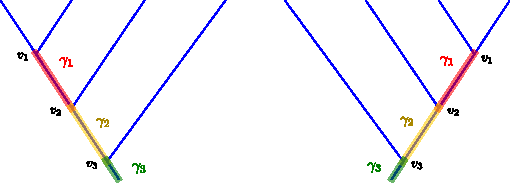
\includegraphics[scale=1]{figures/Example_SL2LusztigCycles.pdf}
		\caption{The Lusztig cycles $\{\g_i\}$ for the two Demazure weaves $\s_1^4\lr\s_1$ used in \Cref{ex:dual_Lusztig_cycles}.(1) and (2). Here $\gamma_i$ denotes the Lusztig cycle associated to the trivalent vertex $v_i$, and an edge highlighted with the corresponding color denotes weight 1 for the corresponding Lusztig cycle. Weave edges not highlighted in the corresponding color denote weight 0 for the corresponding Lusztig cycle.}\label{fig:Example_SL2LusztigCycles}
	\end{figure}
\end{center}

\begin{center}
	\begin{figure}[h!]
		\centering
        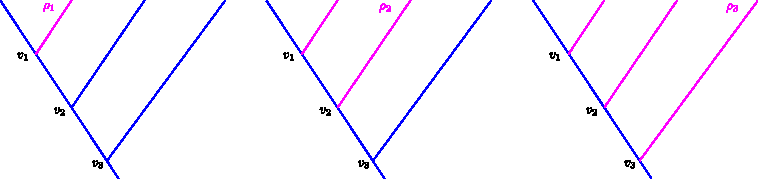
\includegraphics[scale=1]{figures/Example_DualLusztigCycles.pdf}
		\caption{The dual Lusztig cycles $\{\rho_i\}$ for the weave $\w:\s_1^4\lr\s_1$ for \Cref{ex:dual_Lusztig_cycles}.(1). Here $\rho_i$ denotes the dual Lusztig cycle associated to the trivalent vertex $v_i$.}\label{fig:Example_DualLusztigCycles}
	\end{figure}
\end{center}


\begin{example}\label{ex:dual_Lusztig_cycles} (1) Consider the Demazure weave $\w:\beta\to\delta(\beta)$ for $\beta=\s_1^4$ drawn in \cref{fig:Example_DualLusztigCycles}. The Lusztig cycles $\{\g_1,\g_2,\g_3\}$ of $\w$ are depicted in \Cref{fig:Example_SL2LusztigCycles} (left), and the dual Lusztig cycles $\{\rho_1,\rho_2,\rho_3\}$ are depicted in pink in \cref{fig:Example_DualLusztigCycles}, where a pink edge indicates weight 1, and a blue edge indicates weight 0.

\begin{center}
	\begin{figure}[h!]
		\centering
		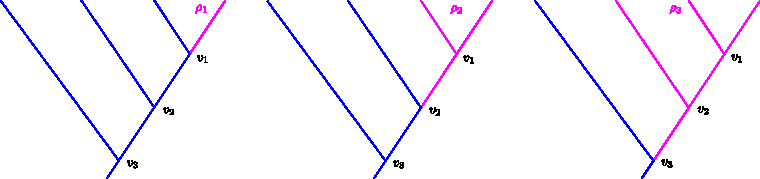
\includegraphics[scale=1]{figures/Example_DualLusztigCycles2.pdf}
		\caption{The dual Lusztig weave cycles $\{\rho_i\}$ from \cref{ex:dual_Lusztig_cycles}.(2), highlighted in pink.}\label{fig:Example_DualLusztigCycles2}
	\end{figure}
\end{center}

Suppose that $\{\g_1,\g_2,\g_3\}$ are given, as in \Cref{fig:Example_SL2LusztigCycles} (left). Verifying that $\rho_1$ is indeed the correct dual Lusztig cycle at $v_1$ is immediate from the definition, as only the clause \Cref{def:dual_Lusztig_cycles}.$(i)$ needs to be applied. To justify $\rho_2$ and $\rho_3$ we also need  \Cref{def:dual_Lusztig_cycles}.$(ii)$, and thus we must first compute certain intersections with the Lusztig cycles in order to apply \eqref{eq:dualLusztigcycle_trivalentrule_left}. Specifically, we can construct $\r_2$ by propagating upwards from the northeast edge of $v_2$, with weight 1. Then we scan the weave upwards until we reach the next vertex, which is the trivalent vertex $v_1$. By \eqref{eq:dualLusztigcycle_trivalentrule_left}, the northwest edge of $v_1$ automatically gets assigned weight 0, as this is the weight that was propagating upwards from $\r_2$ on the south edge $e_\mathsf{s}$ of $v_1$ when we reached $v_1$. By \eqref{eq:dualLusztigcycle_trivalentrule_left}, the weight of $\r_2(e_\mathsf{ne})$ assigned to the northeast edge $e_\mathsf{ne}$ of $v_1$ is given by
$$\rho_2(e_\mathsf{ne})=\rho_2(e_\mathsf{s})+\textcolor{blue}{\langle (\rho_2)_{<v_1},\g_1\rangle}=0+1.$$
Here we have used that $\g_1$ and $(\rho_2)_{<v_1}$ intersect only at the trivalent vertex $v_2$, and with contribution +1, as determined in \Cref{ex:local_intersection}.(1). This shows that $\r_2$ is drawn correctly in \cref{fig:Example_DualLusztigCycles}. Iterating this argument also verifies that $\r_3$ is correct as drawn in \cref{fig:Example_DualLusztigCycles}.\\


\noindent (2) Consider the weave $\w:\beta\to\delta(\beta)$ for $\beta=\s_1^4$ drawn in \cref{fig:Example_DualLusztigCycles2}. The Lusztig cycles are depicted in \Cref{fig:Example_SL2LusztigCycles} (right), and the dual Lusztig cycles in \Cref{fig:Example_DualLusztigCycles2}. In this case, all the correction terms $\langle (\rho_q)_{<v},\g_v\rangle$ appearing in \eqref{eq:dualLusztigcycle_trivalentrule_left} vanish. For instance, $\r_2$ starts at $v_2$ and propagates upwards with weight 1 on the south edge $e_\mathsf{s}$ of $v_1$ when we reach $v_1$. By \eqref{eq:dualLusztigcycle_trivalentrule_left}, the northwest edge of $v_1$ is assigned weight 1, and the weight of $\r_2(e_\mathsf{ne})$ assigned to the northeast edge $e_\mathsf{ne}$ of $v_1$ is given by
$$\rho_2(e_\mathsf{ne})=\rho_2(e_\mathsf{s})+\textcolor{blue}{\langle (\rho_2)_{<v_1},\g_1\rangle}=1+0.$$
Here we have used that $\g_1$ and $(\rho_2)_{<v_1}$ intersect only at the trivalent vertex $v_2$ and with local intersection 0 at $v_2$, cf.~ \Cref{ex:local_intersection}.(1).\\

\noindent (3) More generally, consider an arbitrary $\mbox{SL}_2$ Demazure weave, i.e.~a weave $\w:\sigma_1^n\lr\sigma_1$ consisting of one color $\sigma_1$, always depicted in blue in our diagrams. Suppose that we are propagating a dual Lusztig cycle $\r$ upwards and we reach a trivalent vertex. Let $(\b_\downarrow,{\bf a}_\downarrow)$ be the weighted braid word given by $\r$ on a horizontal slice below (and arbitrarily close to) a trivalent vertex $v$. Let us denote by $(\b_\uparrow,{\bf a}_\uparrow)$ the weighted braid word given by $\r$ on a horizontal slice above (and arbitrarily close to) the trivalent vertex $v$. Since $\r$ starts at some trivalent vertex below $v$, we are interested in propagating $\r$ upwards past $v$, using \eqref{eq:dualLusztigcycle_trivalentrule_left}: that is, we seek a formula for $(\b_\uparrow,{\bf a}_\uparrow)$ in terms of $(\b_\downarrow,{\bf a}_\downarrow)$. For the braid words this is just going from $\b_\downarrow=\ldots\s_{i_k}\ldots$ to $\b_\uparrow=\ldots\s_{i_k}\s_{i_k}\ldots$ for the index $i_k$ corresponding to the trivalent $v$, and in particular the lengths satisfy $\ell(\b_{\uparrow})=\ell(\b_{\downarrow})+1$. In this $\mbox{SL}_2$ case, there is also a simple formula near a trivalent vertex $v$ for the weights. Namely, if ${\bf a}_\downarrow=(\ldots,a_{k-1},a_k,a_{k+1},\ldots)\in\N^{\ell(\b_{\downarrow})}$, where $a_k$ is the weight of $\r$ at the south edge $e_\mathsf{s}$ of $v$, then
\begin{equation}\label{eq:upwards_propagation_SL2}
{\bf a}_\uparrow=(\ldots,a_{k-1},a_k,\textcolor{purple}{\max(a_k,a_{k+1})},a_{k+1},\ldots)\in\N^{\ell(\b_{\downarrow})+1}
\end{equation}
where the newly added entry is highlighted in purple. Here we declare $a_{k+1}=0$ if $i_k$ is the rightmost crossing of $\b_\downarrow$, i.e.~if $k=\ell(\b_\downarrow)$. By comparing to \eqref{eq:dualLusztigcycle_trivalentrule_left}, the term $\max(a_k,a_{k+1})$ in \eqref{eq:upwards_propagation_SL2} is obtained via the sum $\max(a_k,a_{k+1})=a_k+\max(a_{k+1}-a_k,0)$, where $a_k=\r(e_\mathsf{s})$ and $\max(a_{k+1}-a_k,0)=\langle \rho_{<v},\g_v\rangle$ is the correction term. The latter equality is obtained via \Cref{def:locint_3valent} and using that $\g_v$ must end at the other trivalent boundary vertex of $e_\mathsf{s}$, which lies below $v$.
\color{black}

\begin{center}
	\begin{figure}[h!]
		\centering
		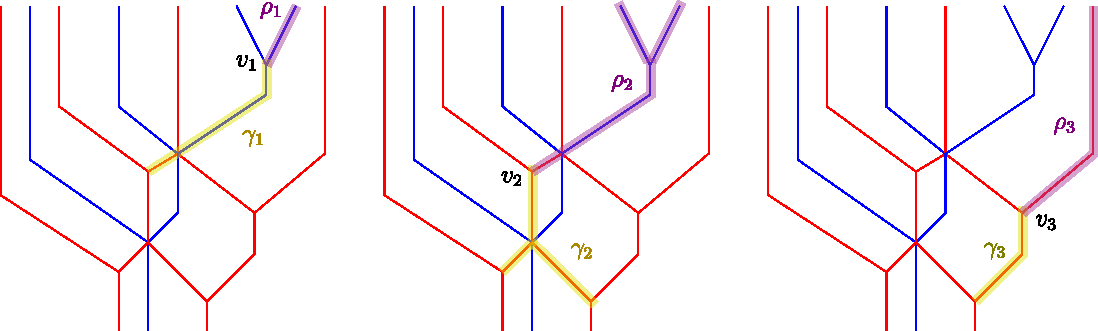
\includegraphics[scale=0.8]{figures/Example_DualLusztigCycles3.pdf}
		\caption{The dual Lusztig cycles $\{\rho_1,\r_2,\r_3\}$ from \cref{ex:dual_Lusztig_cycles}.(4), highlighted in pink, with the corresponding Lusztig cycles $\{\g_1,\g_2,\g_3\}$ highlighted in yellow.}\label{fig:Example_DualLusztigCycles3}
	\end{figure}
\end{center}

\noindent (4) Consider the Demazure weave $\w:\beta\to\delta(\beta)$ depicted in \cref{fig:Example_DualLusztigCycles3}, where $\beta=\s_2\s_1\s_2\s_1\s_2\s_1^2\s_2$. The Lusztig cycles $\g_1,\g_2,\g_3$ associated to the trivalent vertices $v_1,v_2,v_3$ are highlighted in yellow. Specifically, these are all binary weave cycles, with the only values being $0$ and $1$, so we directly highlight the edges where the cycle evaluates to 1. The upwards dual Lusztig cycles $\rho_1,\rho_2,\rho_3$
 are highlighted in purple. Note that there are five Lusztig cycles but $\g_4,\g_5$ have non-zero weights in the bottom boundary. Direct computation also verifies that the corresponding intersections are
$$(\langle\g_i, \rho_j\rangle)=\begin{pmatrix}
1 & 0 & 0\\
0 & 1 & 0\\
0 & 0 & 1
\end{pmatrix},\quad \mbox{for }i,j\in[1,3],$$
with $i=j=1$ being the top left entry and $i=j=3$ the bottom right entry. The only subtle entry is $\langle \g_1,\r_2\rangle=0$, where the intersection is 0 despite the support of the weave cycles geometrically overlapping. Specifically, if $v$ denotes the highest hexavalent vertex, all the three contributions to the intersection number vanish:
$$\langle \g_1,\r_2\rangle=\sharp_{v_1}(\g_1 \cdot \r_2)+\sharp_{v_2}(\g_1 \cdot \r_2)+\sharp_{v}(\g_1 \cdot \r_2)=0+0+0=0.$$
Hence the duality \eqref{eq:duality} holds.\sbs
\end{example}

%%%%%%%%%%%%%%%%%%%%%%%%%%%%%%%%%%%%%
%%%%%%%%%%%%%%%%%%%%%%%%%%%%%%%%%%%%%
%%%%%%%%%%%%%%%%%%%%%%%%%%%%%%%%%%%%%

\subsection{Intersection quiver under weave equivalences and weave mutations}\label{ssec:intersection_Lusztig_cycles_weave_operations} Let $\w,\w':\beta\lr\eta$ be two Demazure weaves, for some braid words $\beta,\eta$. \Cref{def:Lusztig_cycles} provides their collections of Lusztig weave cycles $\{\g_i\}$ and $\{\g'_i\}$, indexed by the corresponding set of trivalent vertices of $\w$ and $\w'$ respectively. \Cref{def:intersection_number}, and see also \Cref{rmk:boundary_intersections}, provides the intersection matrices
$$B_\w=(\langle\g_i,\g_j\rangle),\qquad B_{\w'}=(\langle\g'_i,\g'_j\rangle).$$
The following result explains how $B_\w$ and $B_{\w'}$ are related to each other:

\begin{proposition}\label{prop:intersection_Lusztig_cycles_weave_operations}
Let $\beta,\eta$ be two positive braid words, and $\w,\w':\beta\lr\eta$ two Demazure weaves. Consider the intersection matrices $B_\w$ and $B_{\w'}$ associated to the Lusztig cycles of $\w$ and $\w'$. Then

\begin{enumerate}
    \item If $\w\simeq\w'$ are weave equivalent, there exists a permutation matrix $P$ such that
    \begin{equation}
        B_{\w'}=PB_{\w}P^{-1}.
    \end{equation}
    That is, $B_\w$ and $B_{\w'}$ coincide up to permutation of the indexing of the trivalent vertices.\\

    \item If $\w\stackrel{\mu}{\sim}\w'$ differ by a weave mutation at the $k$th Lusztig cycle, then
\begin{equation}
\langle \gamma'_i,\gamma'_j\rangle =
\begin{cases}
-\langle \gamma_i,\gamma_j\rangle & \text{if } i=k \text{ or } j=k; \\
\langle \gamma_i,\gamma_j\rangle + \langle \gamma_i,\gamma_k\rangle \langle \gamma_k,\gamma_j\rangle & \text{if } \langle \gamma_i,\gamma_k\rangle > 0 \text{ and } \langle \gamma_k,\gamma_j\rangle > 0; \\
\langle \gamma_i,\gamma_j\rangle - \langle \gamma_i,\gamma_k\rangle \langle \gamma_k,\gamma_j\rangle & \text{if } \langle \gamma_i,\gamma_k\rangle < 0 \text{ and } \langle \gamma_k,\gamma_j\rangle < 0; \\
\langle \gamma_i,\gamma_j\rangle & \text{otherwise.}
\end{cases}
\end{equation}
That is, $B_{\w'}$ is obtained by matrix mutation of $B_{\w}$ at the $k$th row and column.
\end{enumerate}
\end{proposition}

\noindent \Cref{prop:intersection_Lusztig_cycles_weave_operations}.(1) is \cite[Corollary 4.31]{CGGLSS25} and \Cref{prop:intersection_Lusztig_cycles_weave_operations}.(2) follows from \cite[Lemma 4.33]{CGGLSS25}. The concept of matrix mutation referred to in \Cref{prop:intersection_Lusztig_cycles_weave_operations}.(2) is explained in \cite[Lemma 2.7.3]{FWZ16}. In the language of quivers, \Cref{prop:intersection_Lusztig_cycles_weave_operations} implies:

\begin{fcor}\label{cor:quiver_cycles_weave_operations}
Let $\beta,\eta$ be two positive braid words, $\w,\w':\beta\lr\eta$ two Demazure weaves. Let $Q_\w$ and $Q_{\w'}$ be the intersection quivers of the Lusztig cycles of $\w$ and $\w'$. Then

\begin{enumerate}
    \item If $\w\simeq\w'$ are weave equivalent, up to vertex relabeling, $Q_{\w'}=Q_\w$.
    
    \item If $\w\stackrel{\mu}{\sim}\w'$ differ by a weave mutation at the $k$th Lusztig cycle, then $Q_{\w'}=\mu_k(Q_\w)$.
\end{enumerate}
\end{fcor}
\vspace{0.2cm}
\noindent In \Cref{cor:quiver_cycles_weave_operations}.(2) we denoted by $\mu_k(Q_\w)$ the mutation of the (ice) quiver $Q_\w$ at its $k$th vertex, which corresponds to the mutable Lusztig cycle $\g_k$. Specifically, $\mu_k(Q_\w)$ is obtained from $Q_\w$ by the following process:
\begin{enumerate}
    \item For each oriented two-arrow $i \to k \to j$ in $Q_\w$ with $i,j$ not both frozen, we add a new arrow $i \to j$.\footnote{If both $i$ and $j$ are frozen, then do nothing.}
    \item Reverse the direction of all arrows in $Q_\w$ incident to the vertex $k$.
    \item Repeatedly remove oriented $2$-cycles, until unable to do so.
\end{enumerate}
\noindent See \cite[Section 2]{FWZ16} for more details on quiver mutation.\\

\noindent The quivers $Q_\w$ obtained as intersection quivers of Lusztig cycles in a Demazure weave $\w$ are reasonably well-behaved. For instance, \cite[Proposition 7.10]{CGGLSS25} implies that, for any Demazure weave $\w$, the quiver $Q_\w$ admits a reddening sequence. The quivers $Q_\w$ are typically of infinite quiver mutation type if $\w$ is an $\SL_n$-weave, $n\geq3$, i.e.~$\beta$ has at least three strands.

%%%%%%%%%%%%%%%%%%%%%%%%%%%%%%%%%%%%%%%%%%%%%%%%%%%%%%%%%%%%
%%%%%%%%%%%%%%%%%%%%%%%%%%%%%%%%%%%%%%%%%%%%%%%%%%%%%%%%%%%%
%%%%%%%%%%%%%%%%%%%%%%%%%%%%%%%%%%%%%%%%%%%%%%%%%%%%%%%%%%%%

\subsection{Lattices}\label{ssec:lattices_seed_data} The $\SA$ and $\SX$-lattices associated to a Demazure weave $\wb$ can be readily named once we introduce braid varieties. Indeed, each Demazure weave $\w$ produces tori $T_\w^\SA$ and $T_\w^\SX$, each embedded in $X(\beta)$, depending on whether it is seen as an $\SA$-scheme or $\SX$-scheme. Then the $\SA$ and $\SX$-lattices for the seed data associated to $\w$ are the character lattices of the respective tori. For now, we emphasize that \textcolor{blue}{the Lusztig cycles span the $\SX$-lattice and the dual Lusztig cycles span the $\SA$-lattice.} The perfect pairing between them, which in particular realizes one as the dual of the other, is given by the intersection form discussed in \Cref{ssec:intersection_cycles}.

%%%%%%%%%%%%%%%%%%%%%%%%%%%%%%%%%%%%%%%%%%%%%%%%%%%%%%%%%%%%
%%%%%%%%%%%%%%%%%%%%%%%%%%%%%%%%%%%%%%%%%%%%%%%%%%%%%%%%%%%%
%%%%%%%%%%%%%%%%%%%%%%%%%%%%%%%%%%%%%%%%%%%%%%%%%%%%%%%%%%%%

\subsection{Demazure weaves from known combinatorics}\label{ssec:Demazure_weaves_from_combinatorics} The literature on algebraic combinatorics and cluster algebras contains many interesting combinatorial models that help manipulate and better understand cluster seeds, e.g.~double wiring diagrams \cite{FZ2000Tests} or $N$-triangulations of surfaces \cite{FG2006}. Central among them are plabic graphs and their alternating strand diagrams, cf.~\cite[Section 11]{Pos}. For instance, the geometry of positroid varieties is intimately connected to the study of reduced plabic graphs, see e.g.~\cite{GL2023,Scott06,SSBW2019}, \cite[Chapter 7]{FWZ16} and references therein. Note also that one can transition from an $N$-triangulation to a plabic graph as in \cite[Section 1.1]{Gon17}.\\

In general, the idea is that one can transition from a plabic graph to a weave by iteratively applying the $T$-shift construction for plabic graphs, cf.~\cite[Section 8.2]{PSBW}. An instance of this is depicted in \Cref{fig:ConjugateSurface10}. This is explained in detail for reduced plabic graphs in \cite[Section 3]{casals2023demazureweavesreducedplabic}, for plabic fences in \cite[Section 3]{casals2022conjugate} and for the more general grid plabic graphs in \cite[Section 3]{CasalsWeng22}. See also \cite[Section 6.1]{casals2025comparingclusteralgebrasbraid}. Intuitively, the weave is the superposition of the plabic graph $\bG$ and all its $T$-iterates. In all the instances above, this construction naturally bijects the bounded faces of $\bG$ with the mutable Lusztig cycles of the corresponding weave $\w(\bG)$. After appropriately choosing base points, the unbounded faces naturally biject to the frozen Lusztig cycles.

\noindent An advantage of using the weave $\w(\bG)$, even when studying $\bG$, is that it is sometimes possible to mutate at the Lusztig cycle $\g(F)$ associated to a face $F$ of $\bG$ and obtain a new weave. This is the case even if the face $F$ was not square. In particular, several seeds in positroids that are {\it not} Pl\"ucker seeds and do not have a description in terms of plabic graphs, can be diagrammatically described via weaves.

\begin{example}
\Cref{fig:ConjugateSurface10} is an illustration of such a phenomenon, where we are effectively mutating at the hexagonal face of a plabic graph $\bG$ for the top positroid variety in $\Gr(3,6)$ and describing the resulting seed in terms of a weave obtained from a weave mutation applied to $\w(\bG)$. Specifically, the initial seed given by the plabic graph $\bG$ at the top left is a Pl\"ucker seed, and the associated weave $\w(\bG)$ obtained by iterated $T$-shifts is depicted at the bottom left. In this case, the mutation at the quiver vertex associated to the hexagonal face results in a non-Pl\"ucker seed for which no plabic graph exists. Nevertheless, the weave $\w(\bG)$ can be mutated within the diagrammatics of Demazure weaves and we obtain a new weave $\mu_{\gamma(F)}(\w)$ describing this non-Pl\"ucker seed. In fact, in this case of the top positroid variety of $\Gr(3,6)$, all cluster seeds can be represented by weaves, cf.~\cite{AnBaeLee21ADE,Hughes21D}.\sbs
\end{example}

\begin{center}
	\begin{figure}
		\centering
		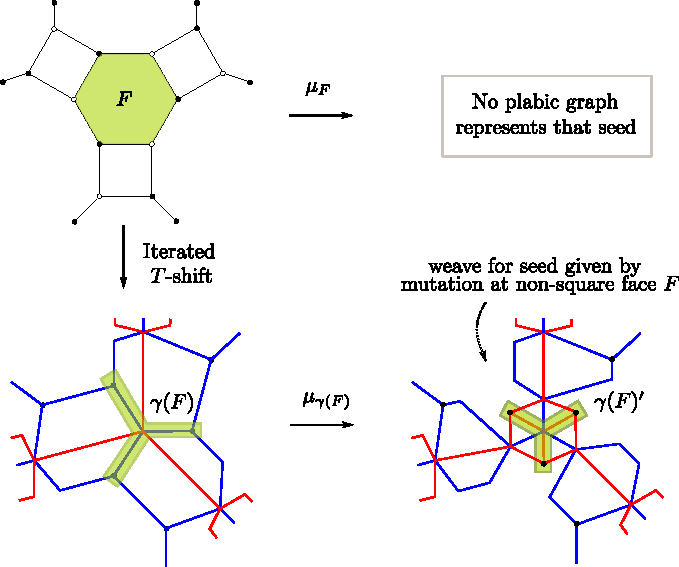
\includegraphics[scale=1]{figures/Gr36_ConjugateSurface10.pdf}
		\caption{(Upper left) A reduced plabic graph $\bG$ for the top positroid variety in $\Gr(3,6)$. If we label the boundary vertices $1, 2, \dots, 6$ clockwise, with the upper right boundary vertex labeled 1, then the cluster variable for the hexagonal face $F$ is $\Delta_{135}$. (Lower left) The weave $\w(\bG)$ corresponding to this plabic graph under iterated $T$-shifts, cf.~\cite{casals2023demazureweavesreducedplabic}. The highlighted Lusztig cycle $\gamma(F)$ corresponds to the face $F$ of $\bG$, and the seed associated to $\w(\bG)$ and its Lusztig cycles is the target seed of that plabic graph. (Lower right) The weave $\mu_{\gamma(F)}(\w(\bG))$ obtained from mutating the weave $\w(\bG)$ at $\gamma(F)$, which corresponds to a mutation of $\Sigma_T(\bG)$ \emph{not} represented by a plabic graph. The new cycle $\gamma(F)'$, corresponding to the vertex where we have mutated, is highlighted. The cluster variable associated to $\gamma(F)'$ is $\Delta_{136}\Delta_{245} - \Delta_{126} \Delta_{345}$, which is not a Pl\"ucker coordinate.}
		\label{fig:ConjugateSurface10}
	\end{figure}
\end{center}

%%%%%%%%%%%%%%%%%%%%%%%%%%%%%%%%%%%%%%%%%%%%%%%%%%%%%%%%%%%%
%%%%%%%%%%%%%%%%%%%%%%%%%%%%%%%%%%%%%%%%%%%%%%%%%%%%%%%%%%%%
%%%%%%%%%%%%%%%%%%%%%%%%%%%%%%%%%%%%%%%%%%%%%%%%%%%%%%%%%%%%

\subsection{Summary of section}\label{ssec:summary_Demazure_weaves} Let $\beta,\eta\in\Br_n^+$ be positive braid words. We have introduced Demazure weaves $\w:\beta\lr\eta$ and their diagrammatic calculus. Such calculus involves:

\begin{enumerate}
    \item The notion of weave equivalences $\w\simeq\w'$ between two weaves $\w,\w':\beta\lr\eta$, cf.~\Cref{def:weave_equivalences}.\\
    \item The notion of weave mutation $\w\stackrel{\mu}{\sim}\w'$ between two weaves $\w,\w':\beta\lr\eta$, cf.~\Cref{def:weave_mutation}.\\
    \item The construction of the Lusztig cycles $\{\g_v\}$ of $\w$, indexed by the trivalent vertices of $\w$, cf.~\Cref{def:Lusztig_cycles}. Similarly, we introduced the dual Lusztig cycles in \Cref{def:dual_Lusztig_cycles}.\\
    \item The construction of a skew-symmetric intersection product for weave cycles, cf.~\Cref{def:intersection_number}. Thus, in particular, the construction of a quiver $Q_\w$ encoding the intersections between the Lusztig cycles $\{\g_v\}$ of $\w$. In addition, \Cref{cor:quiver_cycles_weave_operations} explained how the quiver $Q_\w$ behaves when $\w$ undergoes weave equivalences,  where $Q_\w$ just undergoes a vertex relabeling, and under weave mutation, where $Q_\w$ undergoes a quiver mutation.
\end{enumerate}